	\textbf{Isolation écologique}

	Le chanvre est l'un des plus anciens isolants au monde. Plébiscité pour ses qualités thermiques et acoustiques, il est encore régulièrement utilisé aujourd'hui.

	\hfill \emph{D'après \href{https://www.izi-by-edf-renov.fr/blog/isolation-chanvre}{https://www.izi-by-edf-renov.fr/blog/isolation-chanvre}}

	On souhaite contrôler la qualité d'isolation d'une plaque de laine de chanvre. On dispose pour cela d'un fluxmètre permettant de mesurer le flux thermique à travers la plaque lorsque ses deux faces sont maintenues à des températures différentes : la face \og chaude \fg{} à une température $\theta_{1}$ et la face \og froide \fg{} à une température $\theta_{2}$.

	Le système permettant le maintien de la température de la face \og chaude \fg{} à $25^{\circ}\mathrm{C}$ est arrêté.

	\medskip

	On modélise l'évolution de la température (en ${}^{\circ} \mathrm{C}$) de la face \og chaude \fg{} au cours du temps par une fonction $g$ définie sur $[0 ; +\infty[$ par $g(t)=10 \e^{-\np{0,0045} t}+15$, où $t$ est le temps exprimé en seconde.

	\begin{enumerate}[start=5]
		\item Calculer $\lim\limits_{t \to +\infty} g(t)$.

		\item Montrer que pour tout $t$ de $[0 ; +\infty[$, \quad$ g'(t)=-0,045 \e^{-\np{0,0045} t}$,\quad où $g'$ est la fonction dérivée de la fonction $g$.
	\end{enumerate}

	\needspace{10\baselineskip}

		La courbe représentative de la fonction $g$ (notée $\mathcal{C}_{g}$) ainsi que sa tangente $T$ au point d'abscisse 0 sont représentées dans le repère ci-dessous.

		\begin{center}
		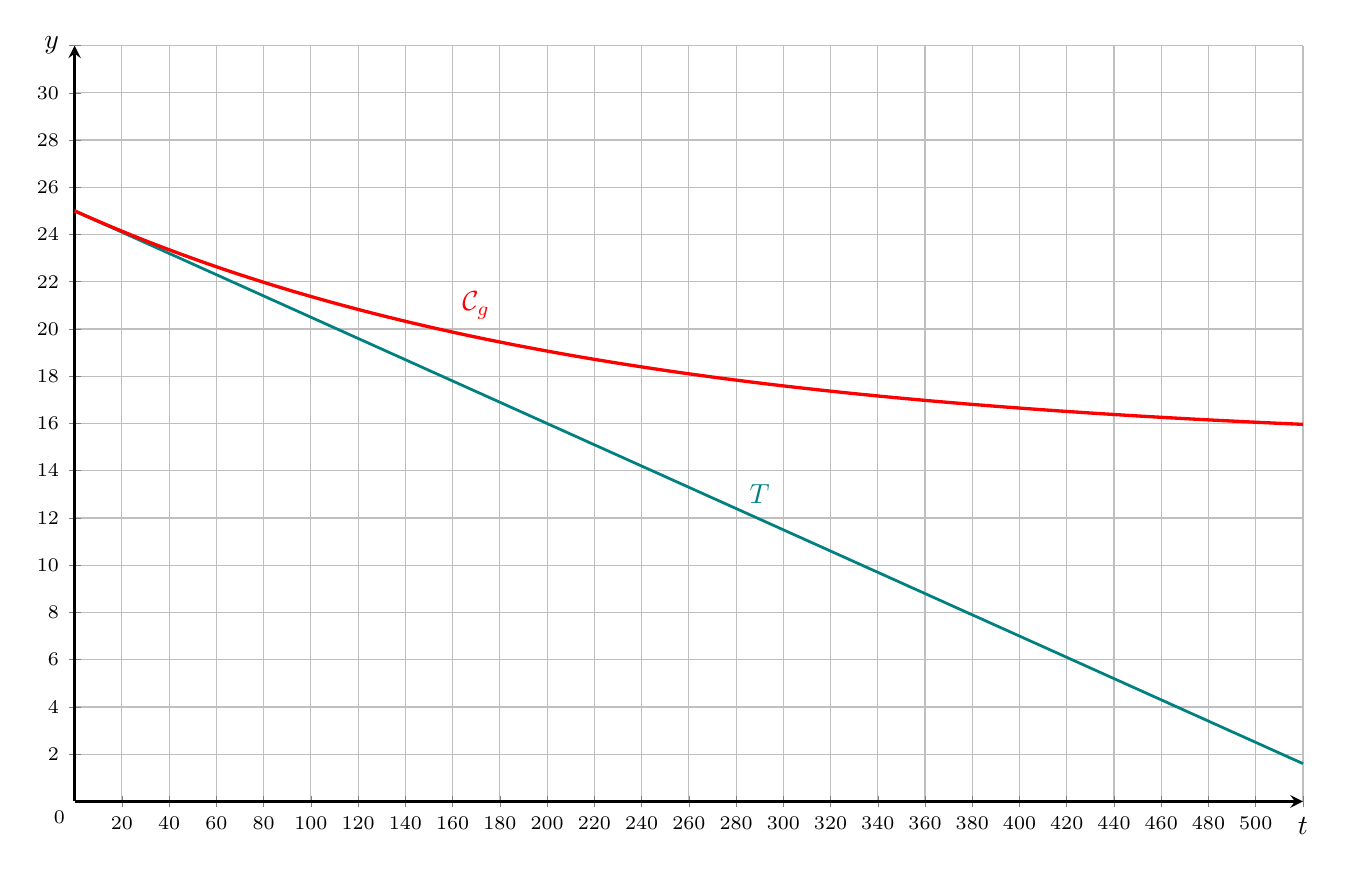
\begin{tikzpicture}
		\begin{axis}[/pgf/number format/.cd, use comma,
			x={0.3mm}, y={3mm},
			xmin = 0, xmax =520 ,
			ymin = 0, ymax =32 ,
			tick label style={font=\scriptsize},
			axis x line =middle, axis y line=middle,
			axis line style={line width=1pt},
			xtick={20,40,...,500}, extra x ticks={520}, extra x tick label={{\normalsize $t$}},
			ytick={2,4,...,30}, extra y ticks={32}, extra y tick label={{\normalsize $y$}},
			clip=false,
			,grid=major]
			\node[below left] at (axis cs: 0,0) {{\scriptsize 0}};
			\addplot [line width=1pt,color=teal,samples=2,domain= 0:520 ]{-0.045*x+25};
			\node[teal] at(axis cs: 290,13) {$T$};
			\addplot [line width=1.2pt,color=red,smooth,samples=100,domain= 0:520 ]{10*exp(-0.0045*x)+15};
			\node[red] at(axis cs: 170,21) {$ \mathcal{C}_g$};
		\end{axis}
		\end{tikzpicture}
		\end{center}


		On admet que la tangente $T$ a pour équation $y=-0,045 t+25$.

		On appelle $\tau$ l'abscisse du point d'intersection de cette tangente avec la droite d'équation $y=15$.
	\begin{enumerate}[resume]
		\item Justifier que 220 est une valeur approchée de $\tau$ à 10 secondes près.

		\item Donner une valeur approchée de $g(\np{1100})$ à $10^{-3}$ près.
	\end{enumerate}

	En physique, on estime qu'à partir d'un temps supérieur à $5 \tau$, la température obtenue est une bonne approximation de la température limite.

	\begin{enumerate}[resume]
		\item Indiquer si le modèle vérifie ce critère.
	\end{enumerate}

\needspace{10\baselineskip}
